\documentclass{report}
\usepackage{pdfpages}
\usepackage{graphicx} 
\usepackage{dirtytalk}
\usepackage{amsmath}
\usepackage{lmodern}
\usepackage{booktabs}
\usepackage{siunitx}
\usepackage{float}
\usepackage{siunitx}
\usepackage[ngerman]{babel}
\usepackage[a4paper, total={6in, 8in}]{geometry}
\begin{document}
\includepdf[pages=-]{./PDFs/Deckblatt_P1.pdf}
\begin{titlepage}
    \begin{center}
        \vspace*{1cm}
            
        \Huge
        \textbf{Auswertung und Protokoll}
            
        \vspace{0.5cm}
        \LARGE
        Zum Versuch STO
        
        \vspace{1.8cm}

        \textbf{Jonas Müther \& Alejandro Schultheiss}
        \vfill
            
        P1 Praktikum\\
       
            
        \vspace{0.8cm}
  

        \vspace{1.8cm}
        \Large
        LMU München \\
        Physik B.Sc.\\
        Deutschland\\
        2026
            
    \end{center}
\end{titlepage}
\tableofcontents

\newpage
\chapter{Vorbereitung}

\section{Versuchsvorbereitung und Grundlagen des Versuchs}

\newpage
\chapter{Durchführung}
\section{Versuchsprotokoll}
\includepdf[pages=3-12]{./PDFs/Versuchsdurchfuehrung.pdf}

\newpage
\chapter{Auswertung}
\section{Teilversuch I: Flugweiten verschiedener Kugeln}

\newpage
\section{Teilversuch II: Elastischer Stoß von Kugeln gleicher \newline Masse}
    \subsection{Theoretischer Hintergrund}
    Im idealisierten Fall des Versuchsaufbaus liegen die Auftreffpunkte der Projektil- und Targetkugel unter Variation des Stoßparameters $b$ jeweils auf Kreisbahnen.
    Der Mittelpunkt dieser Kreisbahnen liegt bei $\vec{M} = \vec{O} + \frac{1}{2} \vec{s}_{zentral}$, wobei $\vec{s}_{zentral}$ die Strecke zwischen Stoßpunkt $\vec{O}$ und Auftreffpunkt der Targetkugel beim Zentralen Stoß beschreibt.
    Der Radius $r_i$ dieser Kreisbahnen ist umgekehrt proportional zur Masse der jeweiligen Kugel $m_i$.
    Es gilt also:
    \begin{equation*}
        \frac{r_{target}}{r_{projektil}} = \frac{m_{projektil}}{m_{target}}
    \end{equation*}
    Somit folgt für $m_{projektil} = m_{target}$, dass die Auftreffpunkte der Kugeln auf dem selben Kreis liegen.
    In unserem Fall mit Kugeln gleicher Masse gilt zudem für den Auftreffpunkt des Flugs ohne Stoß:
    
    \noindent
    \textit{(Dieser muss noch um den Abstand zwischen Rampenende und Stoßursprungspunkt O von 2,5cm vergrößert werden)}
    
    \begin{equation*}
        \vec{s}_{flug} = \vec{s}_{zentral}
    \end{equation*}
    und damit:
    \begin{equation*}
        \vec{M} = \vec{O} + \frac{1}{2} \vec{s}_{flug}
    \end{equation*}
    \subsection{Grafische Analyse der Landepunkte}
    Um die Landepunkte zu visualisieren, wurden die mittleren Landepunkte der Projektil- und Targetkugel bei Variation des Stoßparameters $b$ ausgemessen und in Abbildung \ref*{fig:LandepunkteStoss} dargestellt. Hierzu wurden die jeweiligen durchschnittlichen Landepunkte sowie deren Unsicherheiten mithilfe eines Python-Skripts (matplotlib) in ein Koordinatensystem eingezeichnet.
    Die Kreise um die Landepunkte der Kugeln stellen diese Unsicherheiten dar, welche sich hauptsächlich aus folgenden Aspekten zusammensetzt:
    \begin{list}{-}{}
        \item Streuung der Landepunkte über 4 Durchgänge
        \item Ungenauigkeit des Abtragens des Rampenendes
        \item Messungenauigkeit durch das manuelle Ausmessen mithilfe eines Lineals
        \item Ungenauigkeit beim Schätzen des jeweiligen durchschnittlichen Landepunkts
    \end{list}
    Zusätzlich wurde die theoretisch vorhergesagte Kreisbahn eingezeichnet.
    \newline
    \textit{Anmerkung: Da die Projektilkugel für $b=0$ auf der Vorrichtung für die Targetkugel landet und dann zufällig abprallt, wurde die Koordinate des Projektils für $b=0$ auf den theoretischen Wert von (0, -2) korrigiert.}
    \newpage
    \begin{figure}[H]
        \centering
        \includegraphics[width=1\textwidth]{./Images/LandepunkteStoss.png}
        \caption{Landepunkte der Projektil- und Targetkugel bei Variation des Stoßparameters b}
        \label{fig:LandepunkteStoss}
    \end{figure}
    \newpage
    \subsection{Abweichung von der Theorie}
    Es ist zu erkennen, dass die bestimmten Landepositionen der Projektil- und Targetkugel tatsächlich annähernd auf Kreisbahnen liegen. 
    Jedoch stimmen diese Kreisbahnen nicht vollständig mit der theoretischen Vorhersage überein.
    \newline
    Zunächst fällt auf, dass der Landepunkt der Projektilkugel für $b=0,3 cm$ stark in y-Richtung von der Kreisbahn abweicht, die durch die anderen Messwerte bestimmt wird. Hier ist davon auszugehen, dass dieser Fehler, wie auch für
    $b=0$ durch ein abprallen der Kugel von der Haltevorrichtung für die Targetkugel verursacht wurde.
    Physikalisch deutlich interessanter ist allerdings die generelle Abweichung der Kreisbahnen von Target- und Projektilkugel von der Theorie.
    Für diese Abweichung gibt es mehrere Ursachen, von welchen hier die relevantesten diskutiert werden sollen.

    \subsubsection{Abweichung durch endliche Radien der Kugeln}
    Aufgrund der endlichen Radien der Kugeln findet der Stoß der Kugeln nicht im Punkt O statt. Wie man mithilfe von Abbildung \ref*{fig:Stoss}  erkennen kann ist der Startpunkt der Kugeln abhängig vom Stoßparameter b verschoben.
    \begin{figure}[H]
        \centering
        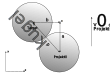
\includegraphics[width=0.4\textwidth]{./Images/Stoß.png}
        \caption{Abweichung der Startpunkte der Kugeln von Punkt O aufgrund der endlichen Radien der Kugeln}
        \label{fig:Stoss}
    \end{figure}
    \noindent
    Entsprechend diser Grafik müssen die gemessenen Landepunkte des Targets um $b$ in x-Richtung und um $a = \sqrt{d_{kugel}^2 - b^2}$ in y-Richtung korrigiert werden.
    Diese korrektur wurde in der folgenden Grafik \ref*{fig:StossKorrigiert} wieder mithilfe des Python-Skripts für jeden Landepunkt durchgeführt.
    \textit{Anmerkung: In der Grafik wurden aus Gründen der Übersichtlichkeit nur die Mittelwerte angepasst, die Messungenauigkeit der Originalwerte gilt allerdings natürlich weiterhin.}
    \begin{figure}[H]
        \centering
        \includegraphics[width=1.0\textwidth]{./Images/LandepunkteStossUndKorrektur.png}
        \caption{Abweichung der Startpunkte der Kugeln von Punkt O aufgrund der endlichen Radien der Kugeln}
        \label{fig:StossKorrigiert}
    \end{figure}
    \newpage
    In der Grafik \ref*{fig:StossKorrigiert} ist zu erkennen, dass diese korrigierten Landepunkte bereits deutlich besser mit der theoretischen Vorhersage übereinstimmen.
    Insebesondere für große Stoßparameter $b$ liegen die korrigierten Landepunkte der Projektilkugel allerdings immer noch relativ deutlich von der Theorie entfernt, was darauf hindeutet, dass es noch weitetere Fehlerquellen gibt,
    die diese Abweichung verursachen.
    Bestimmt man die Abweichung in Abhängigkeit von b mithilfe eines weiteren Python Skripts, so ergibt sich ein Verlauf in Abhängigkeit des Stoßparameters $b$, wie er in Abbildung \ref*{fig:AbweichungKorrigierteLandepunkte} dargestellt ist.
    \begin{figure}[H]
        \centering
        \includegraphics[width=1.0\textwidth]{./Images/AbweichungenKorrigierteLandepunkte.png}
        \caption{Abweichung der korrigierten Landepunkte der Kugeln von der theoretischen Vorhersage}
        \label{fig:AbweichungKorrigierteLandepunkte}
    \end{figure}
    \noindent
    Beobachtet man diesen Verlauf, so fällt auf, die Abweichung der Landepunkt der Targetkugel keine eindeutige Tendenz aufweist. Die Abweichung der Landepunkte der Projektilkugel hingegen nimmt 
    (unter vernachlässigung des Ausreißers für $b=0,3cm$) mit zunehmendem Stoßparameter $b$ zu.
    \newpage
    \subsubsection{Abweichung durch Reibung und Abstand zwischen Rampe und Projektilhalterung}
    Grafik \ref*{fig:AbweichungKorrigierteLandepunkte} zeigt insbesondere, dass die Abweichung der Landepunkte der Projektilkugel vom theoretischen Verlauf mit zunehmendem Stoßparameter
    $b$ deutlich zunimmt. Dies liegt vermutlich unter anderem daran, dass die Gleitreibung während des Stoßes eine große Rolle spielt. Diese führt dazu,
    dass die Kugeln, welche mit zunehmendem Stoßparameter $b$ länger aneinander entlang gleiten, stärker abgebremst werden und so eine geringere Flugweite
    erreichen.    
    

    \noindent
    Hinzu kommt, dass infolge der Geometrie des Versuchsaufbaus das Projektil für größere Stoßparameter eine größere Strecke zwischen Rampe und Targetkugel unter Einfluss der Erdbeschleunigung zurücklegt,
    bevor es die Targetkugel trifft. Dies führt dazu, dass die Targetkugel tiefer getroffen wird(Siehe Abbildungen \ref*{fig:Tieferer Stoss} und \ref*{fig:Noch Tieferer Stoss}), 
    was dazu führt, dass die Projektilkugel eine größere Komponente in negative z-Richtung erhält. 
    Hierdurch verkürzt sich die Flugweite, weshalb der Fehler mit zunehmendem Stoßparameter $b$ zunimmt.
    \newline
    Diese Effekte erklären auch, weshalb die Abweichung für die Targetkugel mit zunehmendem Stoßparameter $b$ keine eindeutige Tendenz aufweist.
    Zwar ist auch die Targetkugel von der Gleitreibung betroffen, was eine verkürzung der Flugweite verursacht, 
    allerdings wirkt für die Targetkugel der Effekt, tiefer getroffen zu werden in entgegengesetzter Richtung.
    Da die targetkugel durch einen tieferen Treffer eine größere Komponente in positive z-Richtung erhält, verlängert sich die Flugweite.
    Dadurch könnte es dazu kommen, dass die beiden Effekte sich teilweise gegenseitig aufheben, wodurch keine eindeutige Tendenz der Abweichung erkennbar wird.
    \newpage
    \begin{figure}[H]
        \centering
        
\includegraphics[width=0.8\textwidth]{./Images/StoßWeiterUnten.png}
        \caption{Stoßhöhe für $b=0$}
        \label{fig:Tieferer Stoss}
    \end{figure}
    \begin{figure}[H]
        \centering
        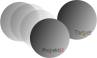
\includegraphics[width=0.8\textwidth]{./Images/StoßNochWeiterUnten.png}
        \caption{Stoßhöhe für $b > 0$}
        \label{fig:Noch Tieferer Stoss}
    \end{figure}
\newpage
\section{Teilversuch III: Bewegungsanalyse mit Hochgeschwindigkeitskamera}

\newpage
\section{Teilversuch IV: Bestimmung der Erdbeschleunigung}

\newpage
\chapter{Anhang}
\section{Python Skripte}

\section{Verwendete Daten}
\subsection{TV I:}
\subsection{TV II:}
\textit{Die folgenden Daten sind alle in cm angegeben.}
    \begin{center}
        \begin{tabular}{c|cccc|cccc}
        & \multicolumn{4}{c|}{Datensatz Projektil} & \multicolumn{4}{c}{Datensatz Target} \\
        Stossparameter b 
        & $x_p$ & $y_p$ & $y_p^{corr}$ & $\Delta r_p$ 
        & $x_t$ & $x_t^{corr}$ & $y_t$ & $\Delta r_t$ \\
        \hline
        0.00  & 0.0 & -2.0 & 0.0  & 0.0 & 0.0   & 0.0   & 26.7 & 0.3 \\
        0.30  & 4.0 & 0.9  & 2.9  & 0.4 & -4.0  & -3.7  & 26.3 & 0.3 \\
        0.40  & 4.9 & -0.7 & 1.3  & 0.3 & -5.4  & -5.0  & 25.9 & 0.3 \\
        0.60  & 7.0 & 0.6  & 2.5  & 0.3 & -7.8  & -7.2  & 24.8 & 0.3 \\
        0.90  & 9.8 & 3.4  & 5.2  & 0.3 & -11.0 & -10.1 & 21.7 & 0.3 \\
        1.20  & 11.8 & 7.4 & 9.0  & 0.4 & -13.3 & -12.1 & 17.7 & 0.3 \\
        1.50  & 11.9 & 12.5 & 13.8 & 0.4 & -13.9 & -12.4 & 12.3 & 0.3 \\
        1.70  & 10.5 & 15.7 & 16.8 & 0.3 & -13.2 & -11.5 & 8.5  & 0.3 \\
        1.80  & 9.3 & 17.7 & 18.6 & 0.4 & -12.0 & -10.2 & 6.1  & 0.5 \\
        1.90  & 7.0 & 19.9 & 20.5 & 0.3 & -9.7  & -7.8  & 3.7  & 0.3 \\
        1.95  & 5.0 & 21.3 & 21.7 & 0.3 & -7.6  & -5.7  & 0.5  & 0.4 \\
        \end{tabular}
    \end{center}
\subsection{TV III:}
\subsection{TV IV:}

\end{document}
